\documentclass{article}

\usepackage{hyperref} % for \url{}
\usepackage{listings} % for source code
\usepackage{syntax} %for typesettings BNF grammars
\usepackage{graphicx} %for screenshots

\begin{document}

\title{SAGA User Manual}
\date{}

\maketitle

\section{Introduction}
SAGA is a run-time verifier for Java programs.  During execution of a Java program, SAGA intercepts method calls and method returns (``events'').  Which events are monitored is determined by a communication view, see Section~\ref{sec:views}. SAGA then checks whether the trace of calls and returns conforms to a specification, given by the user.

Attribute grammars are specifications, see Section~\ref{sec:grammars}.  The underlying context-free grammar determines the order in which events should occur,  in other words: the context-free grammar specifies the desired control-flow of a Java program.  Attributes define properties of the data-flow of the program,  and assertions over these attributes specify the desired values of the attributes.

\section{Communication Views}
\label{sec:views}
A communication view is a partial mapping which assigns a terminal (name) to an event. The terminals are used in the grammar (the grammar productions determine the valid orderings between terminals).  Partiality allows filtering out irrelevant events: only events that are mapped to a terminal are monitored.  The EBNF syntax of communication views is as follows:


\begin{grammar}
<View> ::=  LocalView: "local" "view" <Identifier> "grammar" <Filename> "specifies" <ClassOrInterfaceType> "{" (  <LocalTokenDef> ",")+ "}"
\alt GlobalView: "global" "view" <Identifier> "grammar" <Filename>                                   "{" ( <GlobalTokenDef> ",")+ "}"
  ;

<Filename> ::= "/"? (<Identifier> "/")+ ("." <Identifier>)?
  ;

<LocalTokenDef> ::=  <InEvent> <Identifier>
\alt <OutEvent> <Identifier>

<GlobalTokenDef> ::= <OutEvent> <Identifier>

<InEvent> ::= InCall: ("call" | "return") "ExcludeSelfCalls"? <MethodHeader>
\alt  InCons: <ConsHeader>

<OutEvent> ::= OutCall: ("call" | "return") "ExcludeSelfCalls"? <GlobalMethodHeader>
\alt OutCons: ("call" | "return") <GlobalConsHeader>
  
<GlobalMethodHeader> ::= <Modifier>* <MethodRes> <ClassOrInterfaceType> "." <MethodDeclarator> <Throws>?
  
<ConsHeader> ::= <Modifier>* "new" "(" <FormalParameters> ")" <Throws>?
  
<GlobalConsHeader> ::= <Modifier>* <ClassOrInterfaceType> "." "new" "(" <FormalParameters> ")" <Throws>?
\end{grammar}

The syntax of the unspecified non-terminals (like $Identifier$, $FormalParameters$ (a comma-separated list of formal parameters), $Modifier$, $MethodHeader$ etc) is that of Java.

There are two types of views: local and global views.  A local view selects the relevant events that occur in the history of a \emph{single object} (i.e. the history ``local'' to that object).  The type of that object is given after the ``specifies'' keyword.  A global view selects events that occur anywhere in the Java program during execution (i.e. events from a ``global'' history).  The method name ``new'' is reserved to refer to constructors. For an example of a local communication view,  see \lstinline+src/main/specifications/nl/cwi/saga/breader/spec/BReader.view+ in the BufferedReader project.  The PingPong project contains an example global communication view.

A global view contains $OutEvent$s: in addition to the method signature to be monitored, the class or interface type containing the method must also be named explicitly (since there can be multiple classes containing the same signature method).  A local view contains also $InEvent$s.  An $InEvent$ refers to a call or return of a method implemented by the object under consideration.  Since this is always the same type (namely that given after the ``specifies'' keyword in the view declaration), only the method signature should be given.


\section{Attribute Grammars}
\label{sec:grammars}
SAGA currently uses ANTLR v3 \cite{antlr.07} to generate a Java parser for the attribute grammar.  This means two things: grammars must be given in ANTLR 3 syntax,  and all features (and limitations) supported by ANTLR can be used inside the grammars.  See the BufferedReader and PingPong example grammars for a general template.

In addition to the fact that grammars must conform to the ANTLR syntax,  the following rules apply:
\begin{itemize}
\item The start non-terminal of the grammar must be named ``start''.
\item All user-defined types (classes or interfaces) that appear in the communication view must be imported in an @header section in the ANTLR grammar.  This includes parameter types, return types, and types named in outgoing events (see Section~\ref{sec:views} for details).
\item The methods \lstinline+recoverFromMismatchedToken+ and \lstinline+recoverFromMismatchedSet+ must be overridden in a @parser::members section, and RecognitionExceptions must be caught and thrown in an @rulecatch section (see the example \lstinline+BReader.g+ grammar inside the BufferedReader project).
\item Attributes of grammar terminals (i.e. built-in attributes referring to the objects involved in a method call or return) can be accessed by the getters: \lstinline+caller(), callee(), result()+ and \lstinline+name()+, where name is the parameter of the parameter as used in the view.
\item To access attributes of a terminal inside the grammar,  the terminal must be dereferenced to the correct type.  If the view is called BReaderHistory, and the view contains an event called \lstinline+CLOSE+ referring to a call to the \lstinline+close+ method, then the type is:\lstinline+((BReaderHistoryAspect.call_close)$CLOSE+. If the the \lstinline+CLOSE+ event instead referred to returns of \lstinline+close+, then the type is: \lstinline+((BReaderHistoryAspect.call_close)$CLOSE)+.
\end{itemize}

\section{Usage}
%There are two ways to use and compile the code generated by SAGA: manually, or using an automated build process through a Maven project.  Both approaches have Rascal as a prerequisite:
To compile the BufferedReader and PingPong projects, we use Maven.
All dependencies used inside the Maven project are available from Maven's central repository, except the Rascal artefact. Prerequisites:
\begin{itemize}
\item Rascal 0.6.2.201405101911 (Command-Line version). See \url{http://www.rascal-mpl.org/} for the official homepage and \url{https://github.com/cwi-swat/saga/lib} for the Rascal JAR\footnote{The official homepage offers only the latest version, which is not necessarily backwards compatible}.
\item Quick Sequence Diagram Editor (optional, to visualize error reports). See \url{http://sdedit.sourceforge.net/}.
\end{itemize}
To install the Rascal JAR to the local repository, execute the following command in the directory containing the Rascal JAR (named \lstinline+rascal-0.6.2.201405101911.jar+):
\begin{lstlisting}
mvn org.apache.maven.plugins:maven-install-plugin:2.5.1:install-file  \
-Dfile=rascal-0.6.2.201405101911.jar \
-DgroupId=org.rascalmpl \
-DartifactId=rascal-shell \
-Dversion=0.6.2.201405101911 \
-Dpackaging=jar
\end{lstlisting}
Both the BufferedReader and the PingPong project can then be compiled and packaged by executing (inside the folder with \lstinline+pom.xml+):
\begin{lstlisting}
mvn clean package
\end{lstlisting}
The BufferedReader, which takes the location of a file ``FILEPATH'' as a parameter, can then be executed by:
\begin{lstlisting}
java -cp target/lib/antlr-runtime-3.4.jar: \
target/lib/aspectjrt-1.7.3.jar: \
target/breader-1.0-SNAPSHOT.jar \
-ea nl.cwi.saga.breader.BReader FILEPATH
\end{lstlisting}
The -ea parameter, which enables assertion checking, must be used to turn on SAGA.
Executing the above command should lead to an error reported by SAGA: the grammar specifies that the BufferedReader should be closed by the same object that created it,  but the example client program violates this property.  SAGA will print a counterexample in the form of a sequence diagram.  The sequence diagram can be visualized the Quick Sequence Diagram Editor (be sure to enable Edit \textgreater\ Slack mode)

To create your own project, take the BufferedReader project as a template and adjust the path to the specifications (view+attribute grammar) by changing the value of the property \lstinline+rascal.target+ in \lstinline+pom.xml+.  When executing your program, make sure to add the ANTLR and AspectJ JARs to your classpath (using the -cp parameter, see the example above).

%\subsection{Manual Compilation}
%\label{sec:manual-compilation}
%It is also possible to compile manually.  For manual compilation, in addition to Rascal, the following prerequisites must be installed.
%\begin{itemize}
%\item Java JDK version 1.5 or higher. See \url{https://www.java.com/}.
%\item AspectJ version 1.6 or higher.  See \url{http://eclipse.org/aspectj/}.
%\item ANTLR 3, version 3.2 or higher\footnote{ANTLR v4 is not supported (yet)}. See \url{http://www.antlr3.org/}.
%\end{itemize}
%
%After these prerequisites are installed, the BufferedReader example can be compiled by following the below steps.
%\begin{enumerate}
%\item Compile the Java code containing the class or interface to be tested as usual (i.e. however it is compiled normally).
%\begin{lstlisting}
%TODO
%\end{lstlisting}
%
%\item Generate Java source for a Parser and Lexer for the grammar using ANTLR.
%\begin{lstlisting}
%TODO
%\end{lstlisting}
%
%\item Generate an aspect from the communication view using Rascal.
%\begin{lstlisting}
%TODO
%\end{lstlisting}
%
%\item Compile the Generated aspect, the Java Parser and Lexer using AspectJ.
%\begin{lstlisting}
%TODO
%\end{lstlisting}
%
%\item Execute the project.  Make sure to add the JARs of ANTLR and AspectJ (aspectjrt.jar) to your classpath when running the program.
%\begin{lstlisting}
%TODO
%\end{lstlisting}
%\end{enumerate}


\section{Eclipse Plugin}
There is an Eclipse project of SAGA which allows editing of communication views with
syntax highlighting.  The project uses the Rascal Eclipse plugin for parsing.
Follow the below steps to use the SAGA eclipse project:
\begin{enumerate}
  \item Install Eclipse for RCP and RAP Developers and the Rascal Eclipse plugin. See \url{http://www.rascal-mpl.org/start/} for detailed instructions.
  \item Download SAGA project ZIP-file from Github (click ``Download ZIP'' on \url{https://github.com/cwi-swat/saga})
  \item Import the ZIP as a new Eclipse project:
      \begin{enumerate}
         \item Right click in the Package Explorer
         \item Click Import\ldots
         \item Select General \textgreater\ Existing project into workspace \textgreater\ Next
         \item Select archive file and browse to the ZIP
         \item Click Finish
      \end{enumerate}
  \item In the newly imported project ``Saga'', in the package explorer, double click the file src \textgreater\ GeneratorEclipse.rsc
  \item Right click in the text editor that opens and select Start Console. A command prompt rascal\textgreater\ is opened.
  \item Execute the following commands:
\begin{lstlisting}
    rascal>import GeneratorEclipse;
    ok

    rascal>enableSyntaxHighlighting();
    ok
\end{lstlisting}
  \item Open the file with your communication view from the Eclipse package explorer.  The view is syntax highlighted automatically upon opening:
  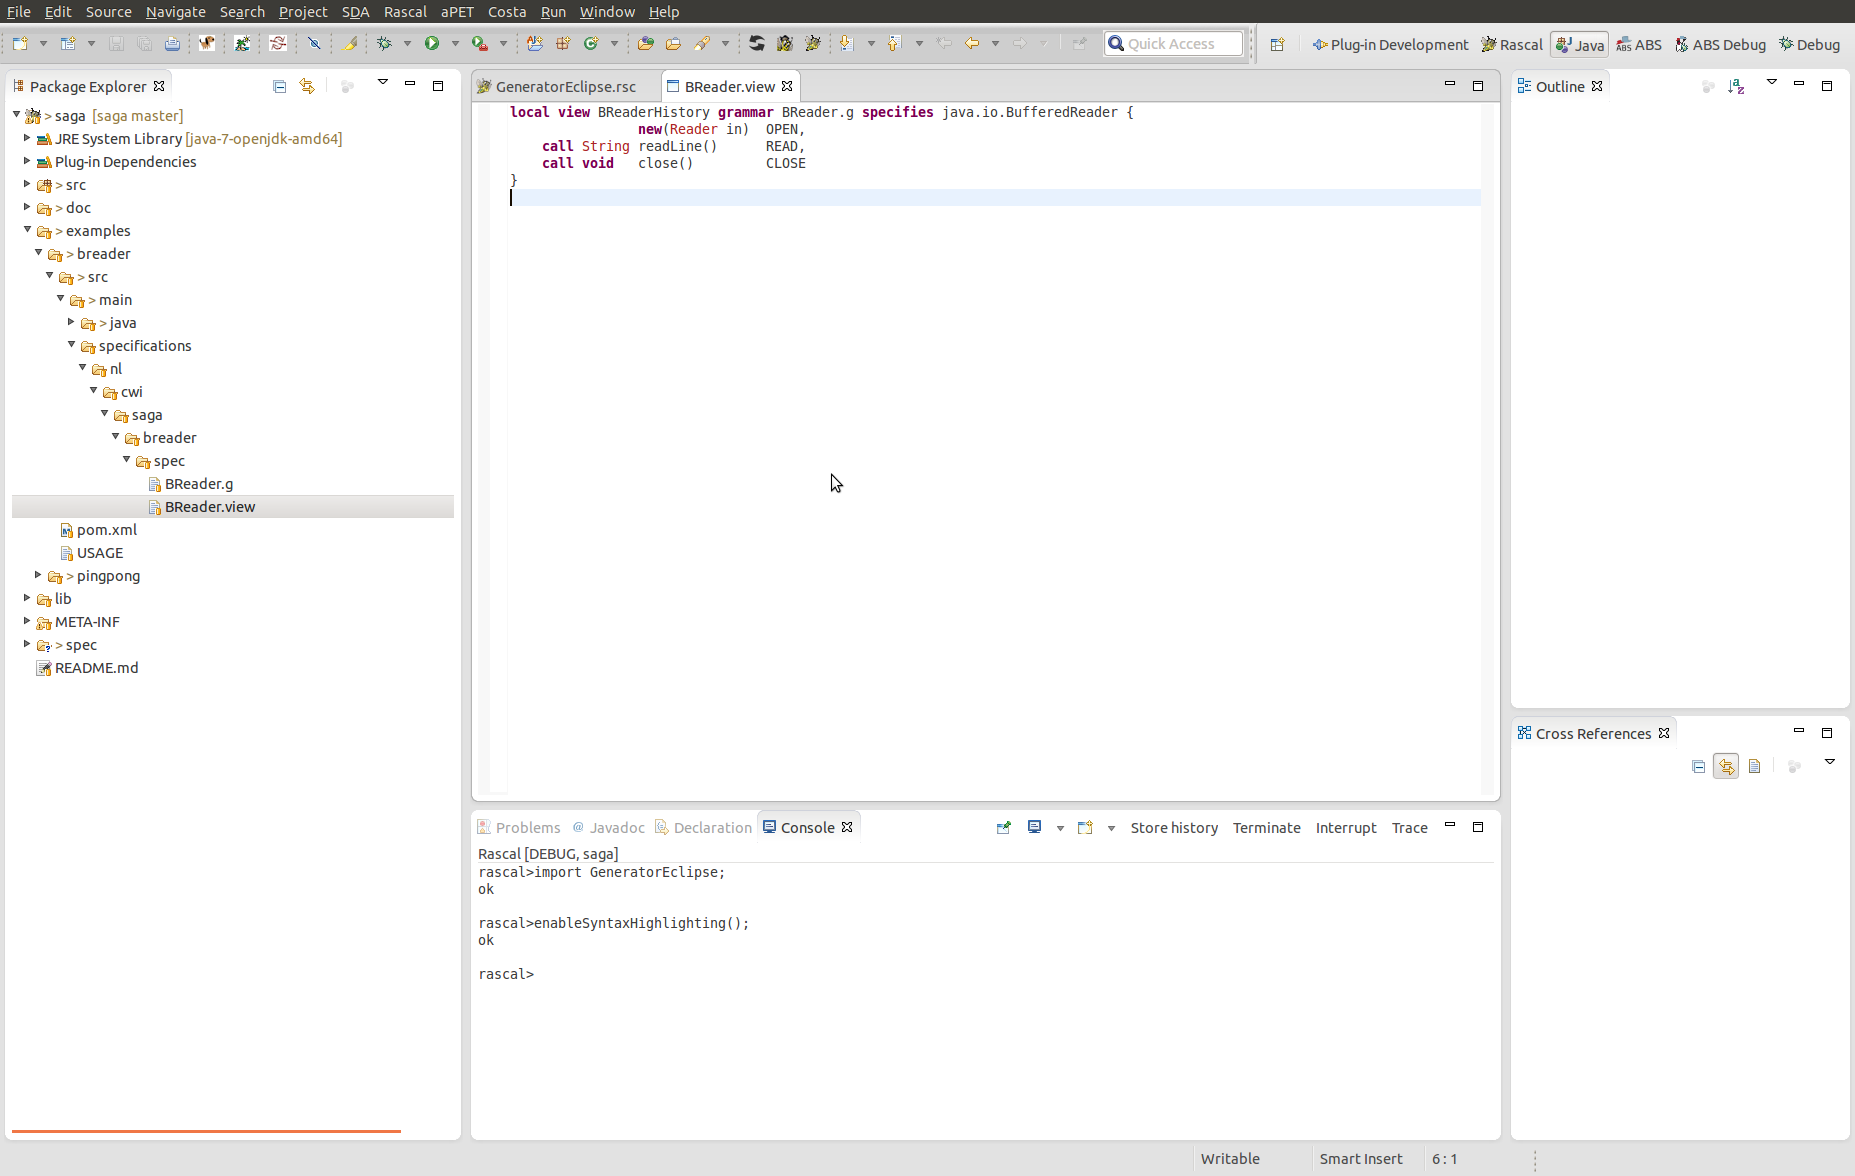
\includegraphics[scale=0.2]{syntaxHighlighting}
\end{enumerate}



\bibliographystyle{abbrv}
\bibliography{manual}

\end{document}